\documentclass[]{article}
\usepackage{lmodern}
\usepackage{amssymb,amsmath}
\usepackage{ifxetex,ifluatex}
\usepackage{fixltx2e} % provides \textsubscript
\ifnum 0\ifxetex 1\fi\ifluatex 1\fi=0 % if pdftex
  \usepackage[T1]{fontenc}
  \usepackage[utf8]{inputenc}
\else % if luatex or xelatex
  \ifxetex
    \usepackage{mathspec}
  \else
    \usepackage{fontspec}
  \fi
  \defaultfontfeatures{Ligatures=TeX,Scale=MatchLowercase}
\fi
% use upquote if available, for straight quotes in verbatim environments
\IfFileExists{upquote.sty}{\usepackage{upquote}}{}
% use microtype if available
\IfFileExists{microtype.sty}{%
\usepackage{microtype}
\UseMicrotypeSet[protrusion]{basicmath} % disable protrusion for tt fonts
}{}
\usepackage[margin=1in]{geometry}
\usepackage{hyperref}
\hypersetup{unicode=true,
            pdftitle={Insert Title},
            pdfauthor={Enter Name},
            pdfborder={0 0 0},
            breaklinks=true}
\urlstyle{same}  % don't use monospace font for urls
\usepackage{graphicx,grffile}
\makeatletter
\def\maxwidth{\ifdim\Gin@nat@width>\linewidth\linewidth\else\Gin@nat@width\fi}
\def\maxheight{\ifdim\Gin@nat@height>\textheight\textheight\else\Gin@nat@height\fi}
\makeatother
% Scale images if necessary, so that they will not overflow the page
% margins by default, and it is still possible to overwrite the defaults
% using explicit options in \includegraphics[width, height, ...]{}
\setkeys{Gin}{width=\maxwidth,height=\maxheight,keepaspectratio}
\IfFileExists{parskip.sty}{%
\usepackage{parskip}
}{% else
\setlength{\parindent}{0pt}
\setlength{\parskip}{6pt plus 2pt minus 1pt}
}
\setlength{\emergencystretch}{3em}  % prevent overfull lines
\providecommand{\tightlist}{%
  \setlength{\itemsep}{0pt}\setlength{\parskip}{0pt}}
\setcounter{secnumdepth}{0}
% Redefines (sub)paragraphs to behave more like sections
\ifx\paragraph\undefined\else
\let\oldparagraph\paragraph
\renewcommand{\paragraph}[1]{\oldparagraph{#1}\mbox{}}
\fi
\ifx\subparagraph\undefined\else
\let\oldsubparagraph\subparagraph
\renewcommand{\subparagraph}[1]{\oldsubparagraph{#1}\mbox{}}
\fi
\usepackage[labelfont=bf, margin=2in]{caption}
\usepackage{floatrow}
\floatsetup[table]{capposition=top}

%%% Use protect on footnotes to avoid problems with footnotes in titles
\let\rmarkdownfootnote\footnote%
\def\footnote{\protect\rmarkdownfootnote}

%%% Change title format to be more compact
\usepackage{titling}

% Create subtitle command for use in maketitle
\newcommand{\subtitle}[1]{
  \posttitle{
    \begin{center}\large#1\end{center}
    }
}

\setlength{\droptitle}{-2em}
  \title{Insert Title}
  \pretitle{\vspace{\droptitle}\centering\huge}
  \posttitle{\par}
  \author{Enter Name}
  \preauthor{\centering\large\emph}
  \postauthor{\par}
  \predate{\centering\large\emph}
  \postdate{\par}
  \date{Insert Date}

\begin{document}
\maketitle

\subsection{Abstract}\label{abstract}

Here you will provide a one-paragraph summary of the experiment.

\subsection{Methods}\label{methods}

See apendix 5A for a sample for what the methods section of your lab
report should look like.

\subsection{Results}\label{results}

The results section should include text describing your results and any
figures or tables that you might like to include. I have included
example code for including two tables and a scatter plot as part of your
results section. You may or may not want all of these.

\subsection{Discussion}\label{discussion}

See appendix 3C and page 5.2 for information on how to write your
discussion.

Example of writing an equation or molecular formula
\(H_2O + CO_2 \rightarrow H_2CO_3\)

\subsection{Calculation}\label{calculation}

Here is where you put in either your calculations, using equations or
inserting a picture of your calcualtions.

For a good source of writing mathematical equation symbols, see
\url{http://www.rpi.edu/dept/arc/training/latex/LaTeX_symbols.pdf}
Example: \(5M*5L=5 moles Fe\)

A figure can be inserted by using the following format, so long as the
picture is saved in the same folder as the Rmarkdown file. NOTE: You
don't have the picture named below, so this markdown file won't knit to
PDF until you either delete line 70 or change the picture to be a
picture in your markdown folder.

\clearpage

\begin{figure}[htbp]
\centering
\includegraphics{iron.jpg}
\caption{Caption of Photo}
\end{figure}

\clearpage

\begin{table}[ht]
\centering
\parbox{2.7in}{\caption{A lovely caption for the table}} 
\begin{tabular}{|r|r|}
  \hline
\textbf{New Iron Label} & \textbf{New Absorbance Label} \\ 
  \hline
0 & 0 \\ 
   \hline
    2.5 & 0.00316 \\ 
   \hline
      5 &   0.006 \\ 
   \hline
     10 &   0.012 \\ 
   \hline
     20 &   0.024 \\ 
   \hline
\end{tabular}
\end{table}

\begin{figure}[htbp]
\centering
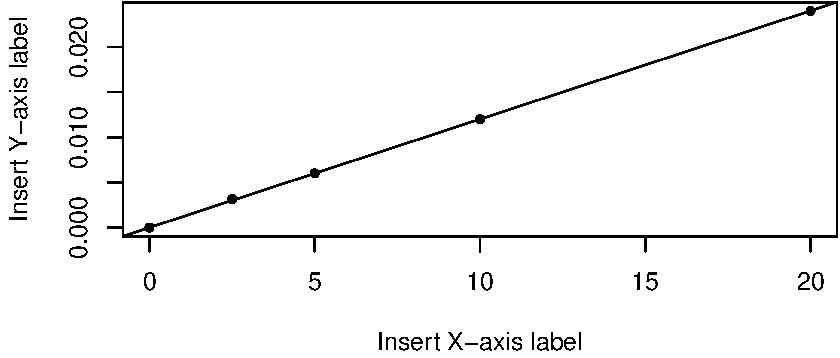
\includegraphics{Iron_Analysis_files/figure-latex/unnamed-chunk-4-1.pdf}
\caption{Insert Caption}
\end{figure}

\begin{table}[ht]
\centering
\parbox{2.7in}{\caption{A lovely caption for the table}} 
\begin{tabular}{|r|r|r|r|}
  \hline
\textbf{New Sample} & \textbf{New Dilute} & \textbf{New Dilute 1 (mg/mL)} & \textbf{New Tablet (mg)} \\ 
  \hline
1 +/- .001 & 100 +/- 1 & 10 +/- .01 & 1000 +/- 10 \\ 
   \hline
\end{tabular}
\end{table}


\end{document}
